\documentclass[../main]{subfiles}
\begin{document}
\chapter{鎖状ネットワークの同期に関する先行研究}
\label{chap:appendix}
\cite{XiaHuang:130506}の解析内容について述べる.

鎖状に無向グラフとして$N$個連なった位相振動子ネットワークのふるまいを以下で記述するとする.
\begin{align}
    \begin{split}
        \dot{\theta}_1&=\omega_1,\\
        \dot{\theta}_i&=\omega_i+\lambda\sin(\theta_{i-1}-\theta_i),\ i=2,3,\ldots,N.
    \end{split}
\end{align}
ここで,$\theta_i,\ \omega_i$をそれぞれ端から$i$番目の振動子の位相と固有振動数とする.$\lambda>0$は振動子間の結合強度とする.
このモデルでは端の振動子$1$が固有振動数$\omega_1$をもつ駆動源となり,他の振動子は駆動源に近い方の隣接した振動子と相互作用する.

$\omega_1=2,\ \omega_2=1$とし,他の$\omega_i$をランダムに選択するとして固有振動数を配置し,結合強度を高めていく数値実験を行ったところ,4つのクラスタリングパターンが観測された.
\renewcommand{\labelenumi}{Case  \theenumi}
\begin{enumerate}
    \item \label{enu:case1} 隣接した駆動振動子と同期し局所クラスターが発生する.
    \item \label{enu:case2} 駆動源と同期する振動子が出現する.
    \item \label{enu:case3} 結合強度が小さい間は隣接した駆動振動子と同期し局所クラスターを構成した後,結合強度がある程度大きくなると局所クラスターが消滅する.
    \item \label{enu:case4} 隣接した駆動振動子が駆動源と同期した後,駆動される振動子自体も同期する.
\end{enumerate}
つまり,各振動子とクラスターを構成するのは,隣接した駆動振動子と,駆動源の2つの振動子のみである.
このパターンは,他の鎖状ネットワークでも普遍的であるため,これらのクラスタリングパターンの分岐を考える.

特に$N=3,\ \omega_1=2,\ \omega_2=1$とする.$\omega_3$を変化させたとき全部で4つの領域に分かれた.
\begin{itemize}
    \item $\omega_3\in[1,2]$のとき,結合強度の増加により隣接した駆動振動子と同期する.Case \ref{enu:case1}に相当する.
    \item $\omega_3\in(2,3]$のとき,結合強度の増加により駆動振動子と同期する.Case \ref{enu:case2}に相当する.
    \item $\omega_3\lesssim 1$のとき,結合強度が小さい間は隣接した駆動振動子と同期し局所クラスターを構成した後,結合強度がある程度大きくなると局所クラスターが消滅する.Case \ref{enu:case3}に相当する.
    \item $\omega_3$が$\omega_1,\ \omega_2$両方ともから離れた値のとき,隣接した駆動振動子が駆動源と同期した後,駆動される振動子自体も同期する.Case \ref{enu:case4}に相当する.
\end{itemize}
以上の分岐を調べるため,以下の方程式を考える.
\begin{align}
    \label{eq:3driving}
    \begin{split}
        \dot{\theta}_1&=\omega_1,\\
        \dot{\theta}_2&=\omega_2+\lambda\sin(\theta_1-\theta_2),\\
        \dot{\theta}_3&=\omega_3+\lambda\sin(\theta_2-\theta_3).
    \end{split}
\end{align}
ここで,$\phi_{21}=\theta_2-\theta_1,\ \Delta\omega_{21}=\omega_2-\omega_1$とすると,
\begin{equation}
    \label{eq:phasediff-21}
    \dot{\phi_{21}}=\Delta\omega_{21}-\lambda\sin\phi_{21}
\end{equation}
となる.ここで,両辺の長時間平均$\langle\cdot\rangle$を考える.
$\lambda$が同期が起こらないくらい小さいとき,$\phi_{21}$の確率分布$\rho(\phi_{21},t)$は十分時間が経つと安定分布に収束する.
\begin{equation}
    \rho(\phi_{21},t)=\frac{\Delta\omega_{21}-\lambda\sin\phi_{21}}{C},\quad C:\mathrm{normalization\ constant}
\end{equation}
この確率分布に$\phi_{21}$が従うとして式\eqref{eq:phasediff-21}の$\sin\phi_{21}$を平均する.
すると,以下のようになる.
\begin{equation}
    \langle\sin\phi_{21}\rangle=\frac{\Delta\omega_{21}-\sqrt{(\Delta\omega_{21})^2-\lambda^2}}{\lambda}.
\end{equation}
よって,式\eqref{eq:3driving}より,$\theta_2$の実効振動数が得られる.
\begin{equation}
    \langle\dot{\theta}_2\rangle=\omega_1+\sqrt{(\Delta\omega_{21})^2-\lambda^2}.
\end{equation}
この式より,$\lambda_c=\Delta\omega_{21}$として,$\lambda\geq\lambda_c$のとき$\langle\dot{\theta}_2\rangle=\omega_1$となり,振動子$1$と振動子$2$は同期する.
同様の手順で$\theta_3$の実効振動数が得られる.
\begin{equation}
    \label{eq:effective-approx}
    \langle\dot{\theta}_3\rangle=\langle\dot{\theta}_2\rangle+\sqrt{(\Delta\omega_{32})^2-\lambda^2}.
\end{equation}
ただし,$\Delta\omega_{32}=\omega_3-\langle\dot{\theta}_2\rangle$である.\\
以上より,振動子の同期条件を求めることができる.
振動子$2$と振動子$3$の同期条件は
$\Delta\omega_{21}\geq 0$のとき,
\begin{align}
    \begin{cases}
        -\lambda\leq\Delta\omega_{31}-\sqrt{(\Delta\omega_{32})^2-\lambda^2}\geq\lambda & (\lambda\leq|\Delta\omega_{21}|),\\
        -\lambda\leq\Delta\omega_{31}\geq\lambda & (\lambda>|\Delta\omega_{21}|).
    \end{cases}
\end{align}
$\Delta\omega_{21}< 0$のとき,
\begin{align}
    \begin{cases}
        -\lambda\leq\Delta\omega_{31}+\sqrt{(\Delta\omega_{32})^2-\lambda^2}\geq\lambda & (\lambda\leq|\Delta\omega_{21}|),\\
        -\lambda\leq\Delta\omega_{31}\geq\lambda & (\lambda>|\Delta\omega_{21}|).
    \end{cases}
\end{align}
ここで,$\Delta\omega_{31}=\omega_3-\omega_1$である.
これらの同期条件から,$\omega_c=-\sqrt{2}|\Delta\omega_{21}|+\omega_1$という臨界振動数を境界とする領域$\omega_3\in(\omega_c,\omega_2)$でCase \ref{enu:case2}のような分離が起こることがわかる.

次に,振動子$1$と振動子$3$の同期条件を考える.
$\phi_{31}=\theta_3-\theta_1$とすると,
\begin{equation}
    \dot{\phi}_{31}=\Delta\omega_{31}-\lambda\sin(\phi_{31}-\phi_{21})
\end{equation}
となるから同期の必要条件は,$|\Delta\omega_{31}|\leq \lambda$となる.
また,$\langle\dot{\theta}_3\rangle=\omega_1$の状況を考えると,式\eqref{eq:effective-approx}から,同期の十分条件が求まる.
\begin{equation}
    \omega_3\leq\omega_1+|\Delta\omega_{21}|-\sqrt{(\Delta\omega_{21})^2-\lambda^2}.
\end{equation}

以上の解析から$\omega_3,\lambda$と同期クラスタの関係が図\ref{fig:appendix-bifurcation}として示される.
\begin{figure}[t]
\centering
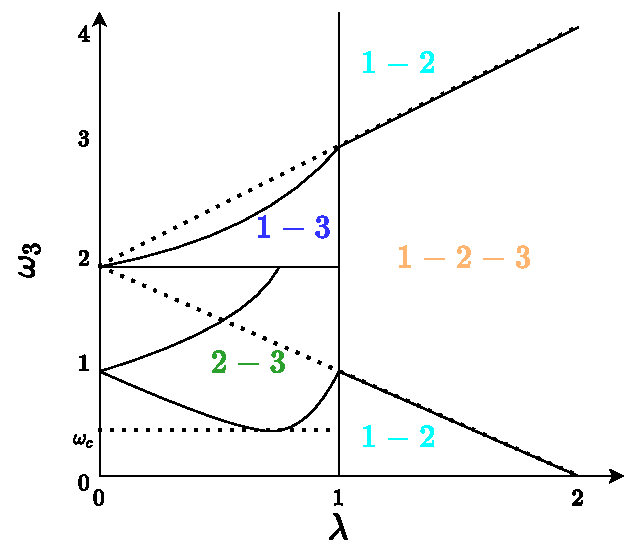
\includegraphics[width=70mm]{./images/appendix-bifurcation.pdf}
\centering
\caption{$\omega_1=2,\ \omega_2=1$のときの固有振動数$\omega_3$と結合強度$\lambda$に対する相図.
あるパラメータ領域で同期クラスタが発生する場合,その振動子の組を各領域に示している.また,同期クラスタが異なるパラメータ領域の境界を実線で示している.}
\label{fig:appendix-bifurcation}
\end{figure}
また,式\eqref{eq:effective-approx}を再帰的に利用することで$N>3$の場合でも同様の解析が可能となる.
\end{document}